\documentclass[floatfix,onecolumn]{aastex631}

\usepackage{amssymb}
\usepackage{amsmath}
\usepackage{microtype}
\usepackage{url}
\usepackage{xspace}
\usepackage{xcolor}
\usepackage{ifxetex}
\ifxetex
\usepackage{fontspec}
\defaultfontfeatures{Extension = .otf}
\fi
\usepackage{fontawesome}



\setlength{\parindent}{3.0ex}


% Projects:
\newcommand{\project}[1]{\textsf{#1}}

\newcommand{\python}{\project{Python}}
\newcommand{\cython}{\project{Cython}}
\newcommand{\cpp}{\project{C++}}
\newcommand{\jupyter}{\project{Jupyter}}

\newcommand{\exoplanet}{\project{exoplanet}}
\newcommand{\lightkurve}{\project{lightkurve}}
\newcommand{\starry}{\project{starry}}
\newcommand{\theano}{\project{Theano}}
\newcommand{\pymc}{\project{PyMC3}}
\newcommand{\celerite}{\project{celerite}}
\newcommand{\dynesty}{\project{dynesty}}
\newcommand{\astroquery}{\project{astroquery}}
\newcommand{\scipy}{\project{scipy}}
\newcommand{\jupytext}{\project{jupytext}}
\newcommand{\sphinx}{\project{sphinx}}
\newcommand{\jupyterbook}{\project{Jupyter-book}}
\newcommand{\arviz}{\project{ArviZ}}
\newcommand{\nbconvert}{\project{nbconvert}}


\newcommand{\tess}{\project{TESS}}
\newcommand{\kepler}{\project{Kepler}}
\newcommand{\gaia}{\project{Gaia}}

\newcommand{\mast}{\project{MAST}}
\newcommand{\exofop}{\project{ExoFOP}}

\newcommand{\tessAtlas}{\project{TESS Atlas}}

% math
\newcommand{\T}{\ensuremath{\mathrm{T}}}
\newcommand{\dd}{\ensuremath{ \mathrm{d}}}
\newcommand{\unit}[1]{{\ensuremath{ \mathrm{#1}}}}
\newcommand{\bvec}[1]{{\ensuremath{\boldsymbol{#1}}}}


\DeclareMathOperator{\invG}{Inv-\mathnormal{\Gamma}}
\DeclareMathOperator{\N}{\mathcal{N}}
\DeclareMathOperator{\U}{\mathcal{U}}
\DeclareMathOperator{\Un}{\mathcal{U}}
\DeclareMathOperator{\Par}{\mathcal{P}ar}
\DeclareMathOperator{\tmin}{\mathnormal{t_{\rm min}}}
\DeclareMathOperator{\tmax}{\mathnormal{t_{\rm max}}}





%% affiliation shortcuts
\newcommand{\SPA}{School of Physics and Astronomy, Monash University, Clayton VIC 3800, Australia}
\newcommand{\OzGravMonash}{OzGrav: The ARC Centre of Excellence for Gravitational Wave Discovery, Clayton VIC 3800, Australia}
\newcommand{\AMNH}{Department of Astrophysics, American Museum of Natural History, New York, NY 10024, USA}
\newcommand{\CCA}{Center for Computational Astrophysics, Flatiron Institute, New York, NY 10010, USA}
\newcommand{\CUNY}{Graduate Center, City University of New York, 365 5th Avenue, New York, NY 10016, USA}
\newcommand{\BMCC}{Department of Science, BMCC, City University of New York, New York, NY 10007, USA}








\newcommand{\atlasUrl}{\href{http://catalog.tess-atlas.cloud.edu.au/}{catalog.tess-atlas.cloud.edu.au}}


\newcommand{\toiTemplateLink}{\href{https://github.com/dfm/tess-atlas/blob/main/src/tess_atlas/notebook_templates/toi_template.py}{github.com/dfm/tess-atlas/.../toi\_template.py}}

\newcommand{\paperPlotsLink}{\github{https://github.com/dfm/tess-atlas/blob/main/paper/figures/make_plots.py}}
\newcommand{\exoplanetOptimization}{\github{https://github.com/exoplanet-dev/pymc3-ext##optimization}}
\newcommand{\exoplanetDocs}{\href{https://docs.exoplanet.codes}{https://docs.exoplanet.codes/}}





%% Confirmed Numbers
% https://exoplanetarchive.ipac.caltech.edu/docs/counts_detail.html
% https://exoplanetarchive.ipac.caltech.edu/index.html
\newcommand{\numConfirmedPlanets}{5,090} % 
\newcommand{\numCandidatesRemaining}{6,959}
\newcommand{\numTessCandidates}{5,488} % 
\newcommand{\numTessPlanets}{227}


%% Atlas numbers
\newcommand{\numAnalysed}{2,833}
\newcommand{\failPercent}{3\%}
\newcommand{\numAnalysedMulti}{357}
\newcommand{\numMultiSystems}{157}
\newcommand{\numAnalysedSingle}{81}
\newcommand{\cpuHrs}{$\sim80,000\ \rm{Hrs}$}

\newif\ifdraft
\drafttrue % switch to false in non-draft version (thereby hiding the todos)
\newcommand{\inDraftVersion}[1]{\ifdraft #1\fi} 


% TODOs
\newcommand{\todo}[3]{\inDraftVersion{{\color{#2}\emph{#1}: #3}}}
\newcommand{\dfmtodo}[1]{\todo{DFM}{red}{#1}}
\newcommand{\avi}[1]{\todo{Avi}{red}{#1}}
\newcommand{\alltodo}[1]{\todo{TODO}{red}{#1}}
\newcommand{\citeme}{{\color{red}(citation needed)}}


\newcommand{\red}{\textcolor{red}}
\newcommand{\textuit}[1]{\textit{\underline{#1}}}



%% Numbers
% https://exoplanetarchive.ipac.caltech.edu/docs/counts_detail.html
% https://exoplanetarchive.ipac.caltech.edu/index.html

\newcommand{\numConfirmedPlanets}{5,090} % 
\newcommand{\numCandidatesRemaining}{6,959}

\newcommand{\numTessCandidates}{5,488} % 
\newcommand{\numTessPlanets}{227}
\newcommand{\numAnalysed}{2,833}
\newcommand{\numAnalysedMulti}{151}
\newcommand{\numAnalysedSingle}{68}
\newcommand{\cpuHrs}{$\sim80,000\ \rm{Hrs}$}

%% links

% % % from: https://github.com/rodluger/corTeX
% % % Add code, proof, and animation hyperlinks
% \definecolor{linkcolor}{rgb}{0.1216,0.4667,0.7059}
% \newcommand{\codeicon}{{\color{linkcolor}\faFileCodeO}}

% % % Define the `oscaption` command for open source figure captions
% \newcommand{\oscaption}[2]{\caption{#2 \codelink{#1}}}


% \makeatletter
\newcommand{\github}[1]{\href{#1}{\textcolor{gray}{\faGithubSquare}}}







% \usepackage[document]{ragged2e}


\setlength{\parindent}{3.0ex}


\newcommand{\ozstar}{\textsc{OzStar}}
\newcommand{\nectar}{\textsc{Nectar}}

\begin{document}

\title{\large\textbf{EoI for software support}:\\Improving the \tessAtlas\ website and catlog-automation}
 

\author{CI: Avi Vajpeyi}
\affiliation{\SPA}

\section*{}
\large{\textbf{What is the \tessAtlas}}\hfill\vspace{0.3em}

The \tessAtlas\ is a catalog of robust parameter estimates and uncertainties on all exoplanet candidates observed by \tess.~\footnote{NASA's Transiting Exoplanet Survey Satellite}
The catalog is hosted on the \nectar\ Research Cloud by Swinburne University of Technology (\atlasUrl). Each exoplanet has its own webpage and \jupyter\ notebook that users can access to study the planet, see Figure~\ref{fig:demo}.

\begin{figure*}
    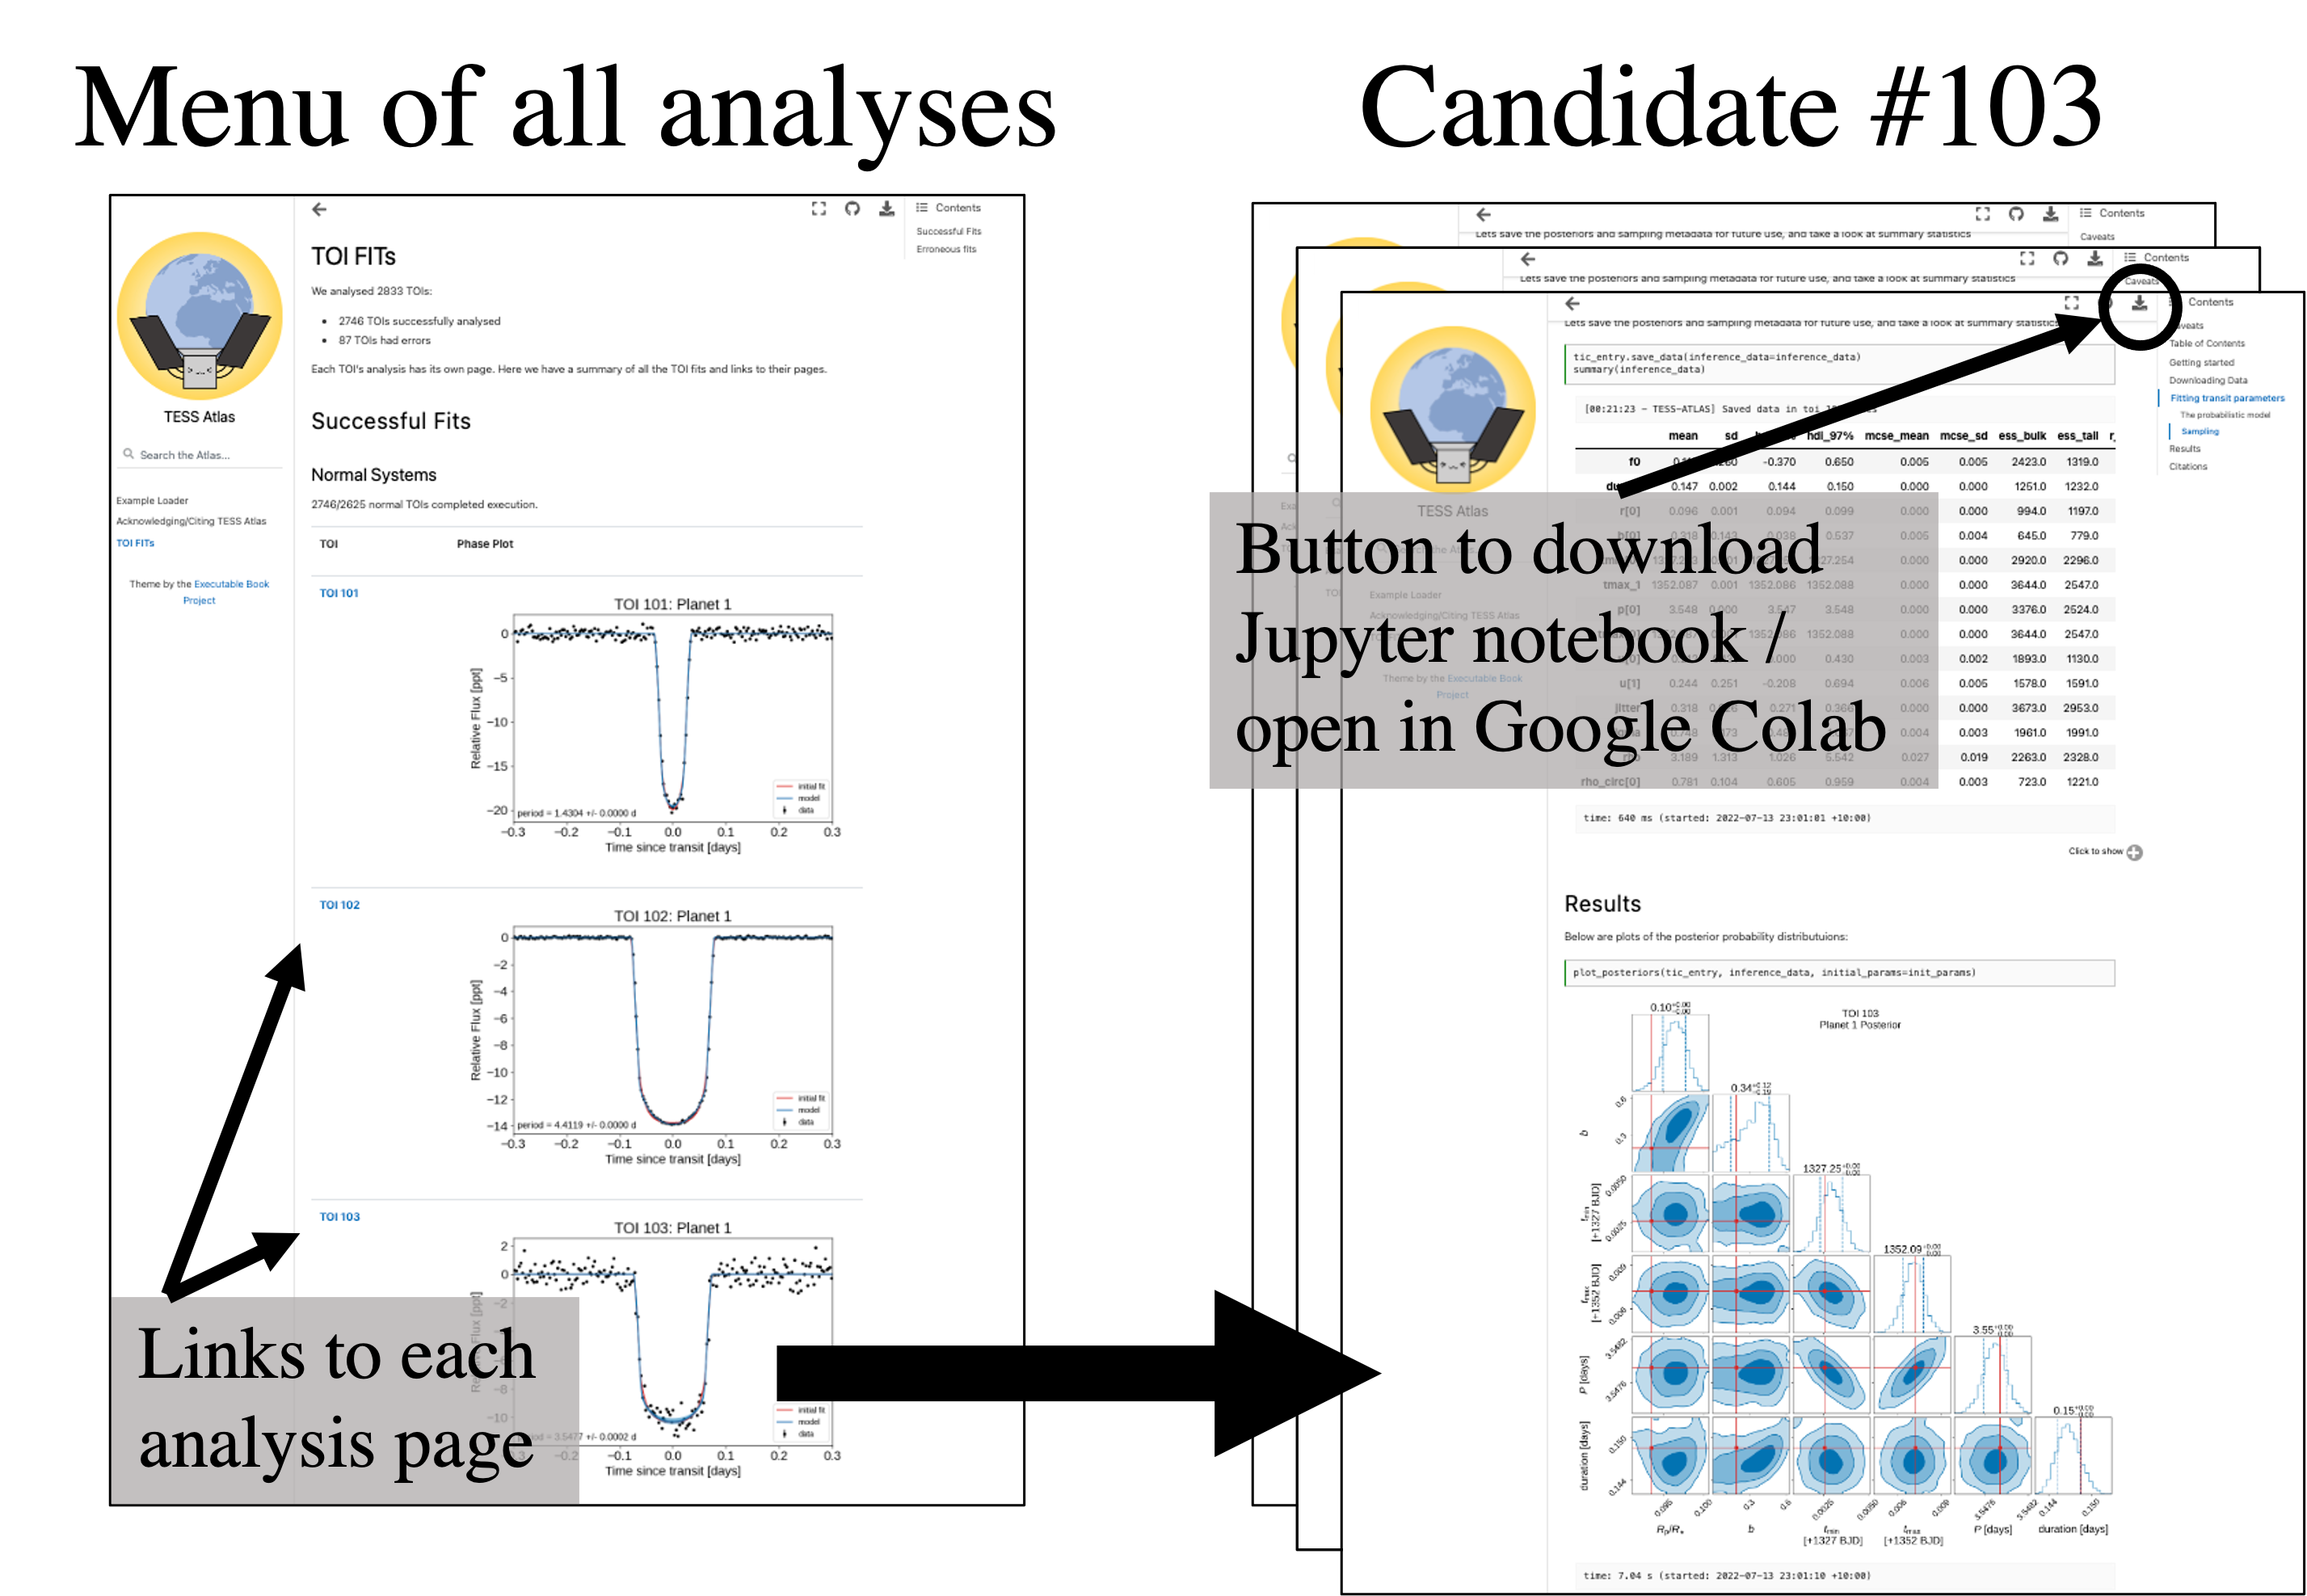
\includegraphics[width=\linewidth]{figures/notebooks_screenshot.png}
    \caption{\textbf{Webpage Example:} (Left) Menu page for all analyses. (Right) Individual analysis.}
    \label{fig:demo}
\end{figure*}



\vspace{1em}


\large{\textbf{Why we need the \tessAtlas}}\hfill\vspace{0.3em}

In March 2022, NASA's exoplanet archive~\citep{Akeson:2013:PASP} surpassed five thousand confirmed exoplanets, a milestone made possible by data from several observatories, including \tess~\citep{Ricker:2015:JATIS, Stassun:2018:AJ, Stassun:2019:AJ, Guerrero:2021:ApJS}.
This list of exoplanets may be dramatically increased once the $\sim6,000$ \tess\ candidates are processed.
Unfortunately, systematic effects and non-planetary astrophysical sources (e.g. stellar granulation and eclipsing binaries) can mimic exoplanet transits~\citep{Rowe:2014:ApJ}.
Hence, to validate these candidates, it is necessary to eliminate false positives and, if possible, conduct additional observations.
Although we have begun to replace manual inspection with objective tests for triage and vetting, we still \underline{rely heavily on human intervention in making dispositions}~\citep{Guerrero:2021:ApJS}.\\



The \tessAtlas\ will:
\begin{enumerate}
    \item aid in the candidate-vetting, promotion and follow-up, 
    \item deliver a starting point for individual analyses, and
    \item provide ensemble population parameters for hierarchical studies.
\end{enumerate}

This is the \underline{first posterior catalog} for \tess\ candidates. Like the \project{Kepler} posterior catalog presented by \citet{Rowe:2014:ApJ}, the \tessAtlas\ will be of great use to the exoplanet community. 

\vspace{1em}


\large{\textbf{ADACS Project Goals}}\hfill\vspace{0.3em}

The \tessAtlas\ analyses run on \ozstar, by processing all exoplanet notebooks in parallel. 
The processed notebooks are then converted into webpages using \jupyterbook\ (a doc generator built on \sphinx).~\footnote{\url{https://jupyterbook.org/}}
We would like ADACS software support/discussion on helping with the following:

\begin{itemize}
    \item \textbf{New candidate Automation:} \tess\ will observe till 2024, and discover new candidate exoplanets weekly. We would like to automate the process of analysing new candidates and updating the website. We are unsure of the best way to set this up on 
    \ozstar\ and \nectar\ (e.g. do we use a cron job to submit \ozstar jobs? How will we trigger the website to update on \nectar?)
    \item \textbf{Alternative to \jupyterbook:} \jupyterbook\ does not perform well in compiling a large number of notebooks into a website (see \href{https://github.com/executablebooks/jupyter-book/issues/1571}{github issue}), and cannot update just one page (e.g. if we want to add one new analysis, we need to rebuild the whole website). Instead of running \jupyterbook\ on the entire catalog, we can run it on each notebook, but then we are unsure of how to nicely structure a menu page, or configure a navigation bar with the same theme (as astronomers, we do not have experience with React etc). Could ADACS help construct an alternative approach?
\end{itemize}

Some guidance/exmaple software from ADACS would greatly help the \tessAtlas\ team improve the catalog.

\newpage

\bibliography{atlas}


\end{document}
